\begin{figure}[!htbp]\centering
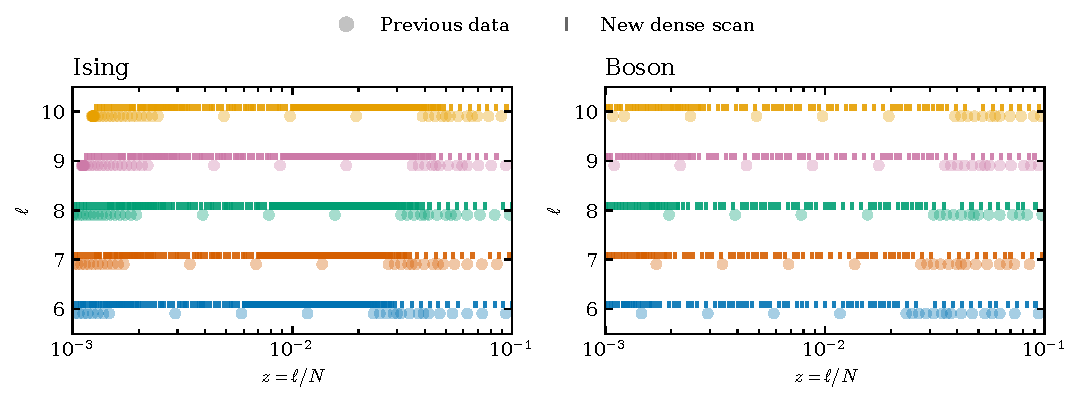
\includegraphics[width=.97\linewidth]{../figs/dense_sampling.pdf}
\caption{Sampling between $10^{-3}$ and $10^{-1}$, common to both interval observables. Circles are the geometries preceding the dense study; vertical marks include the original dense scan and the subsequent fixed-window refinement in Appendix~\ref{sec:common-window-results}. Colors identify $\ell=6,\ldots,10$. Both added grids were chosen from geometry, before their entropies were evaluated, and preserve the largest tested sizes.}
\label{fig:dense-sampling}
\end{figure}

\begin{figure}[!htbp]\centering
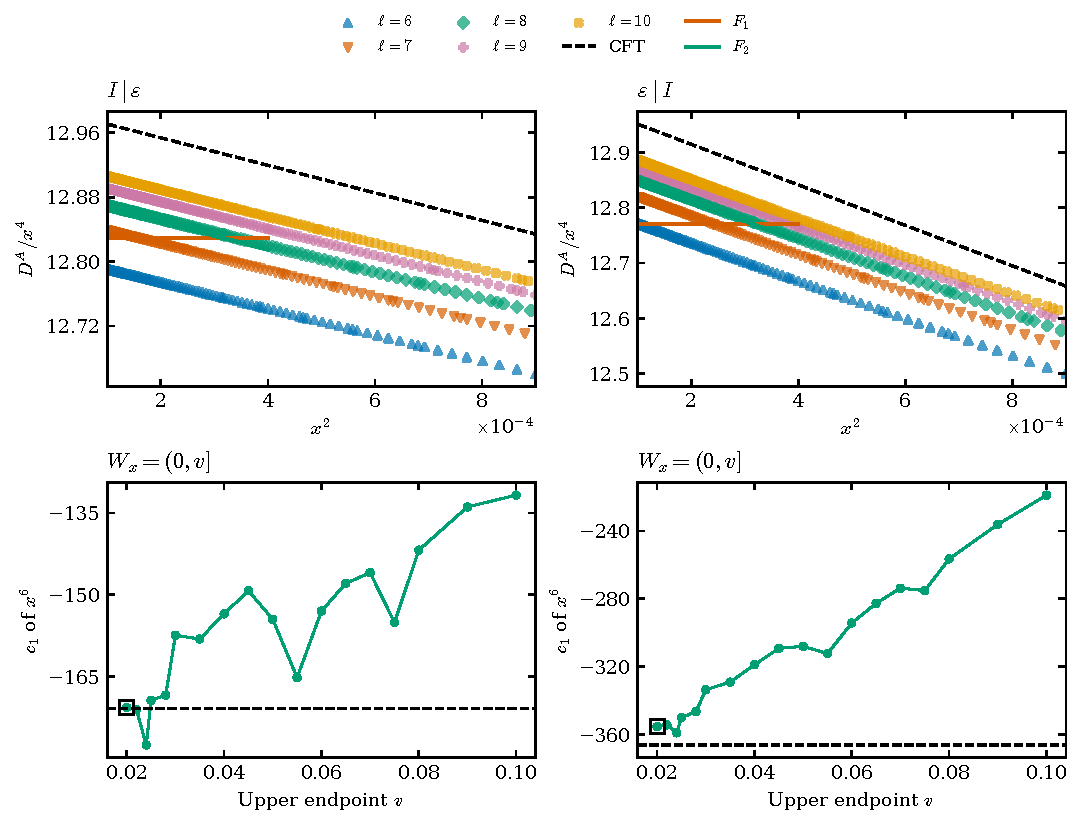
\includegraphics[width=.97\linewidth]{../figs/dense_known_ising.pdf}
\caption{Direct test of the two known Ising second-order coefficients at $p=1/2$. Top: the normalization in Eq.~\eqref{eq:dense-normalized-curve}, zoomed to $0.01\leq x\leq0.03$ with $\ell=6,\ldots,10$, to resolve the fitted slope and the offsets between lengths. The black dashed line is Eq.~\eqref{eq:dense-known-ising}; the fitted lines are drawn only on their actual windows. Bottom: the inferred $x^6$ coefficient as the upper endpoint varies while the displayed lower endpoint stays fixed. Squares mark the reported windows. $I\mid \varepsilon$: $W_x=(0,0.02]$, $m=1255$, $c_0=12.883$, $c_1=-170.71$; $\varepsilon\mid I$: $W_x=(0,0.02]$, $m=1255$, $c_0=12.882$, $c_1=-355.38$. Both $F_2$ coefficients are free; the objective is in $D^A$, not in $D^A/x^4$.}
\label{fig:dense-known}
\end{figure}

\begin{figure}[!htbp]\centering
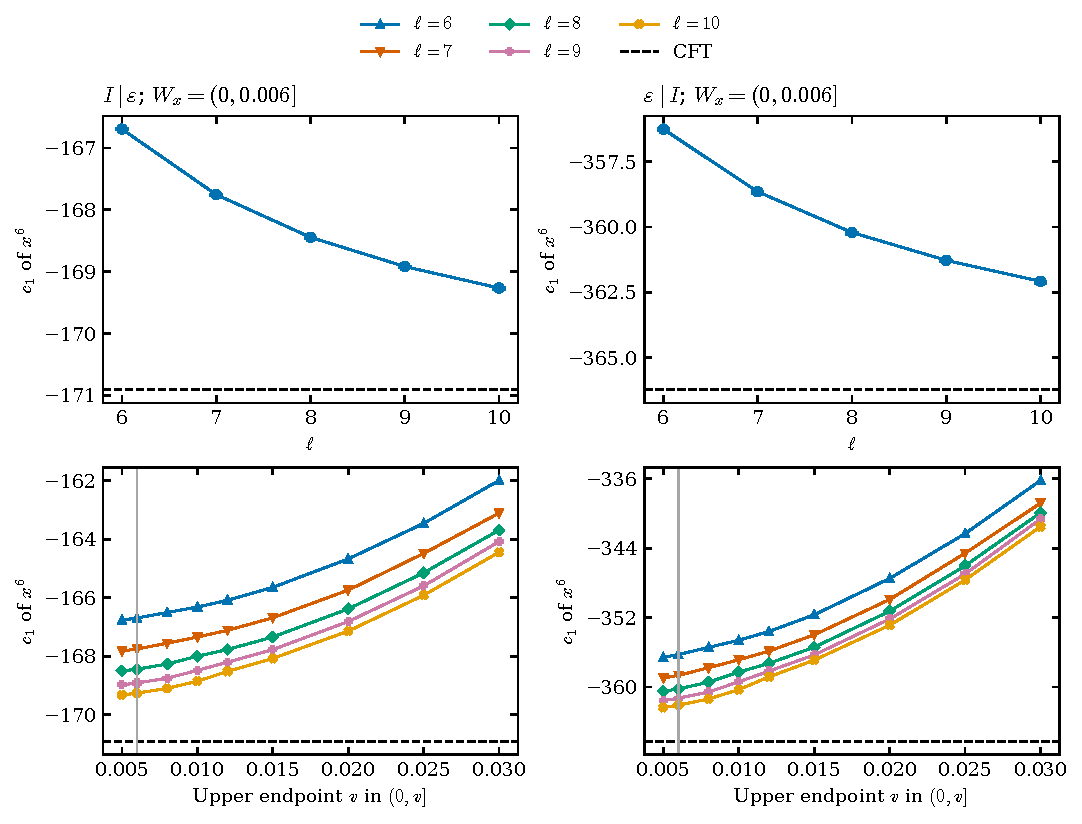
\includegraphics[width=.97\linewidth]{../figs/dense_fixed_subsystem.pdf}
\caption{The same two-power Ising fit performed separately at each subsystem length. Both $x^4$ and $x^6$ coefficients are fitted freely with their exponents fixed; no lattice-correction term is added. Top: vertical bars are the range of $c_1$ across omitted-size refits, not statistical confidence intervals; the marker is the full-data estimate. The black dashed values are Eq.~\eqref{eq:dense-known-ising}. Bottom: coefficient drift as the upper endpoint varies, with each length fitted independently; the vertical line marks the tabulated window. Every fit and every omitted-size training set contains at least forty points. Table~\ref{tab:dense-subsystem} gives the exact counts, both coefficients, and discrepancies.}
\label{fig:dense-subsystem}
\end{figure}

\begin{figure}[!htbp]\centering
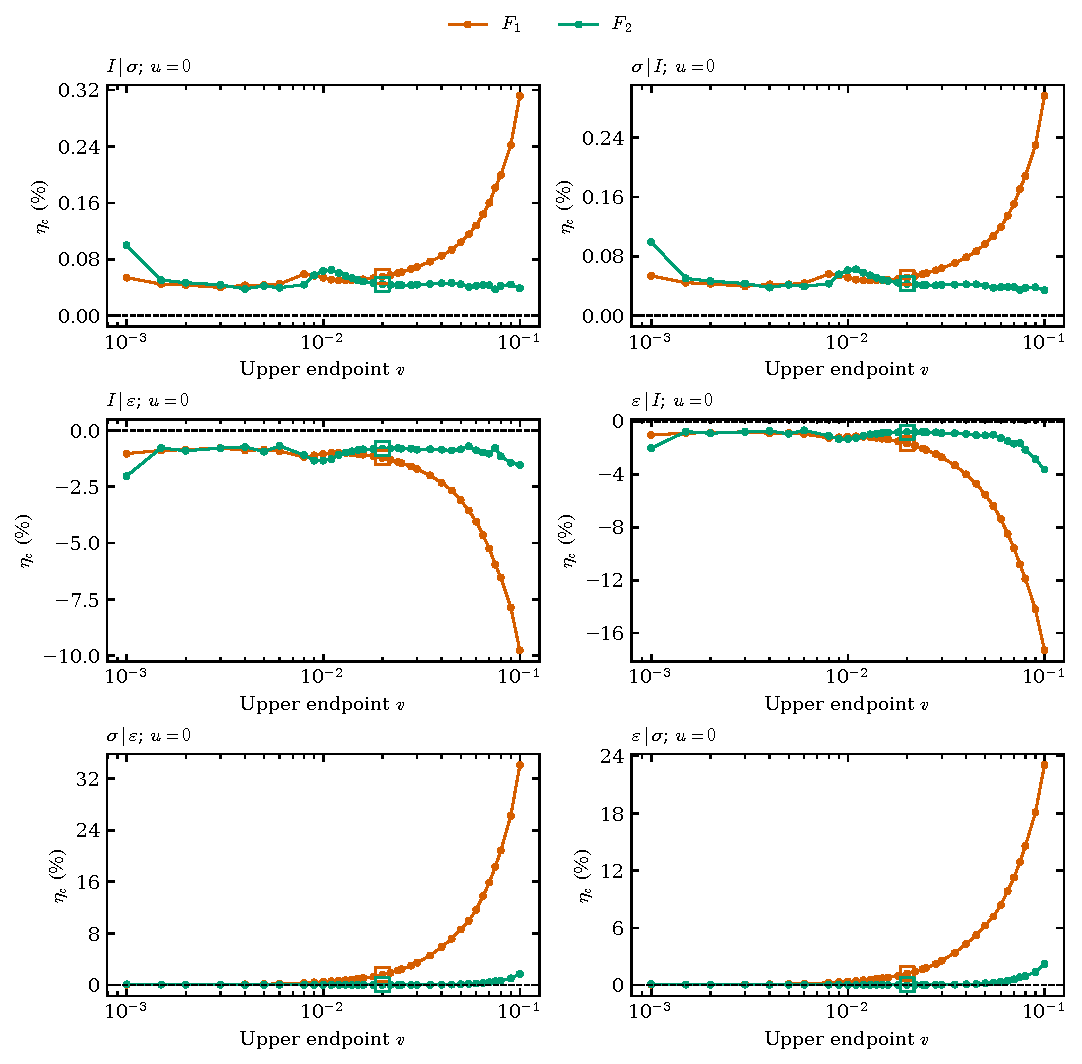
\includegraphics[width=.97\linewidth]{../figs/dense_coefficients_small_ising.pdf}
\caption{Ising small intervals: leading-coefficient discrepancy $\eta_c$ against the upper endpoint $v\leq0.1$ of $W=[u,v]$. Each panel states its fixed $u$; only windows with at least forty points in every omitted-size training set are shown. $F_1$ and $F_2$ always use identical points; $F_2$ fixes both manuscript powers. Squares mark the principal-table windows. All ordinates are linear. The zero line is the theoretical leading coefficient, with its full power of $\pi$.}
\label{fig:dense-coefficients-small-ising}
\end{figure}

\begin{figure}[!htbp]\centering
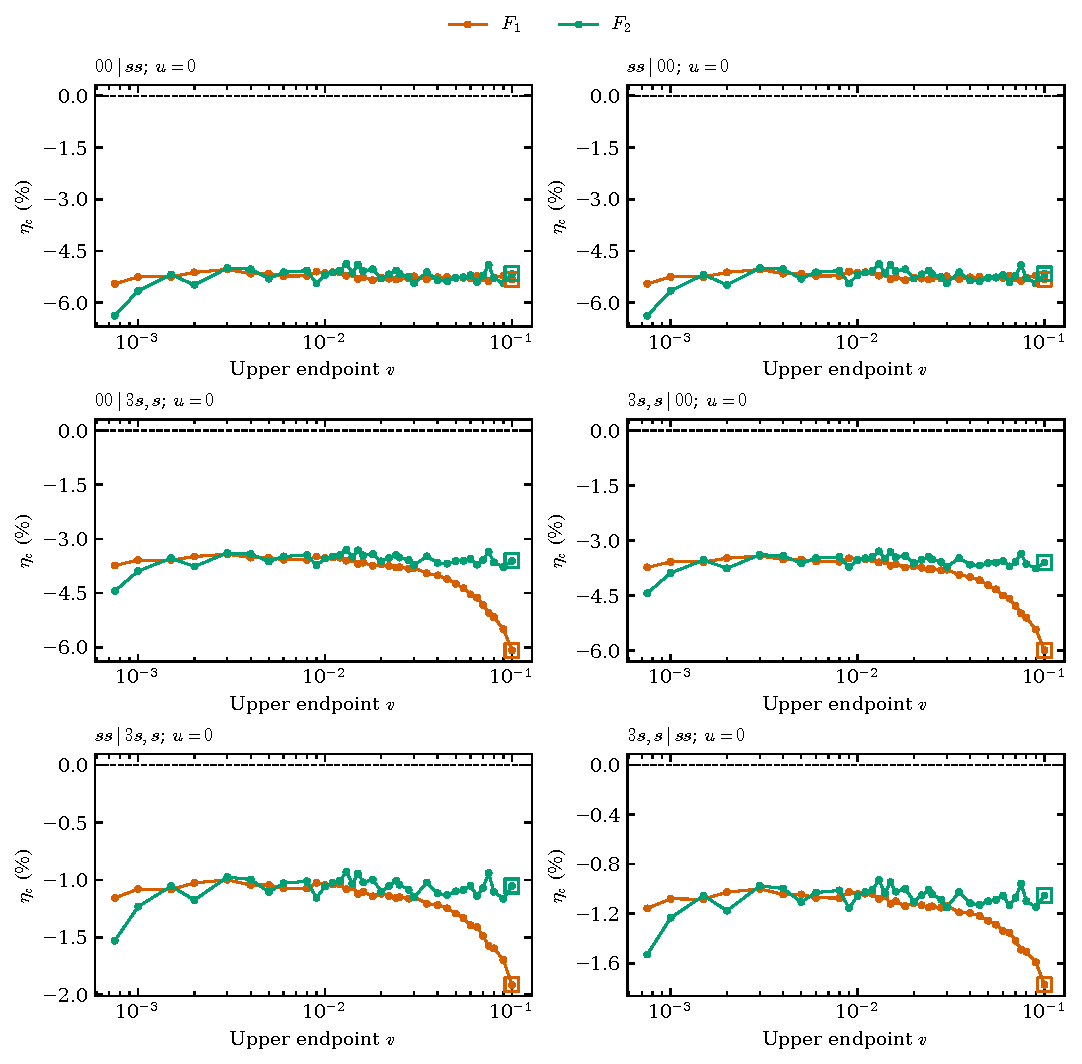
\includegraphics[width=.97\linewidth]{../figs/dense_coefficients_small_boson.pdf}
\caption{Compact boson small intervals: leading-coefficient discrepancy $\eta_c$ against the upper endpoint $v\leq0.1$ of $W=[u,v]$. Each panel states its fixed $u$; only windows with at least forty points in every omitted-size training set are shown. $F_1$ and $F_2$ always use identical points; $F_2$ fixes both manuscript powers. Squares mark the principal-table windows. All ordinates are linear. The zero line is the theoretical leading coefficient, with its full power of $\pi$.}
\label{fig:dense-coefficients-small-boson}
\end{figure}

\begin{figure}[!htbp]\centering
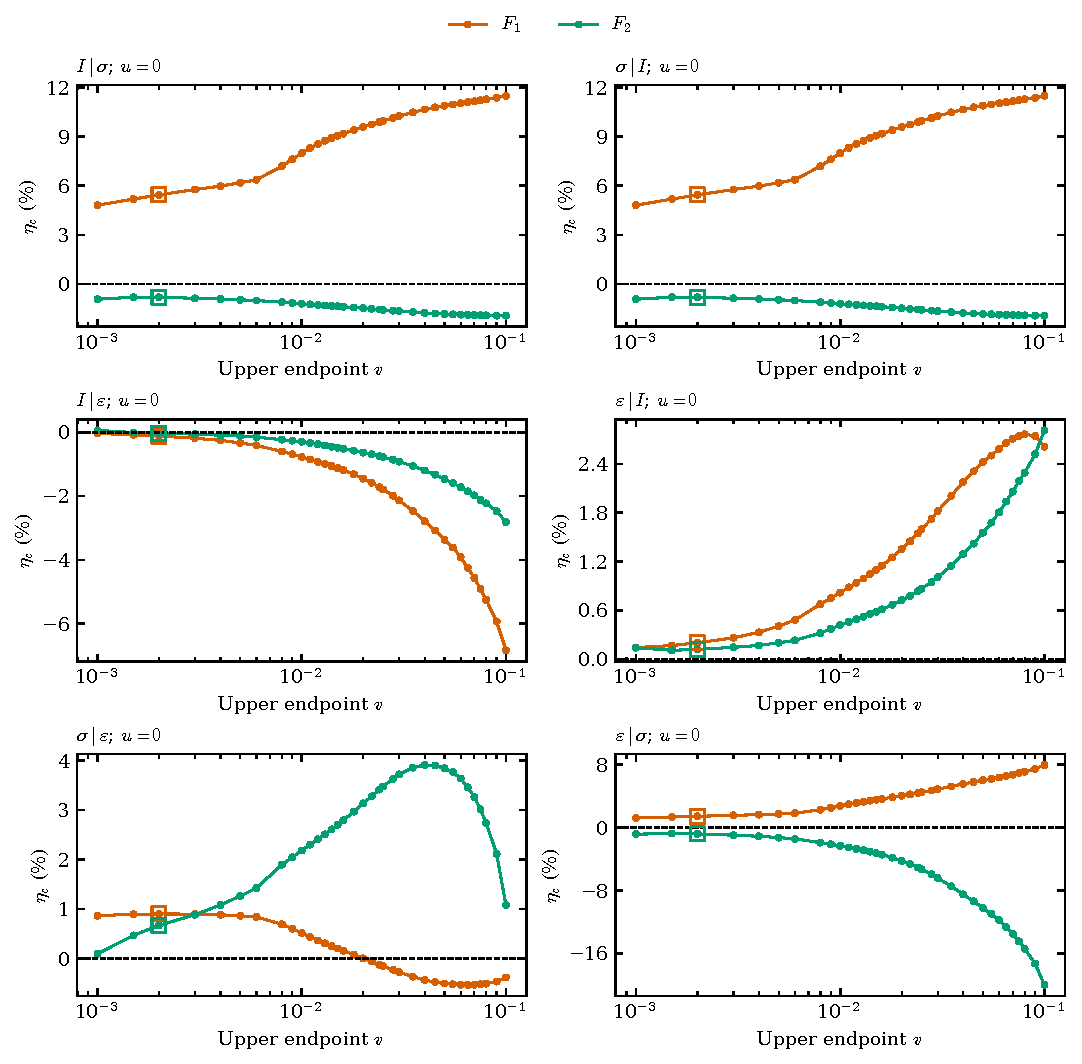
\includegraphics[width=.97\linewidth]{../figs/dense_coefficients_large_ising.pdf}
\caption{Ising large intervals: leading-coefficient discrepancy $\eta_c$ against the upper endpoint $v\leq0.1$ of $W=[u,v]$. Each panel states its fixed $u$; only windows with at least forty points in every omitted-size training set are shown. $F_1$ and $F_2$ always use identical points; $F_2$ fixes both manuscript powers. Squares mark the principal-table windows. All ordinates are linear. The zero line is the theoretical leading coefficient, with its full power of $\pi$.}
\label{fig:dense-coefficients-large-ising}
\end{figure}

\begin{figure}[!htbp]\centering
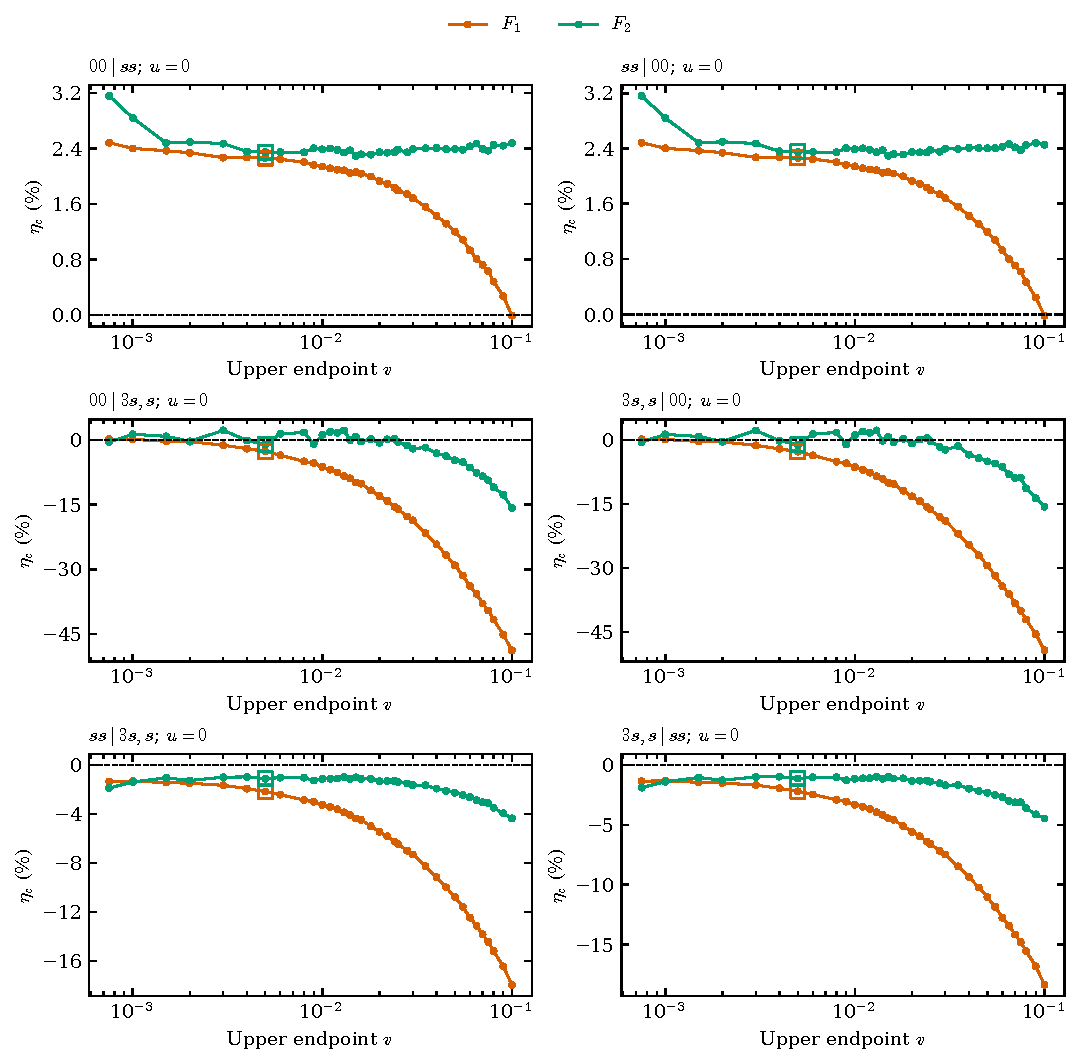
\includegraphics[width=.97\linewidth]{../figs/dense_coefficients_large_boson.pdf}
\caption{Compact boson large intervals: leading-coefficient discrepancy $\eta_c$ against the upper endpoint $v\leq0.1$ of $W=[u,v]$. Each panel states its fixed $u$; only windows with at least forty points in every omitted-size training set are shown. $F_1$ and $F_2$ always use identical points; $F_2$ fixes both manuscript powers. Squares mark the principal-table windows. All ordinates are linear. The zero line is the theoretical leading coefficient, with its full power of $\pi$.}
\label{fig:dense-coefficients-large-boson}
\end{figure}

\begin{figure}[!htbp]\centering
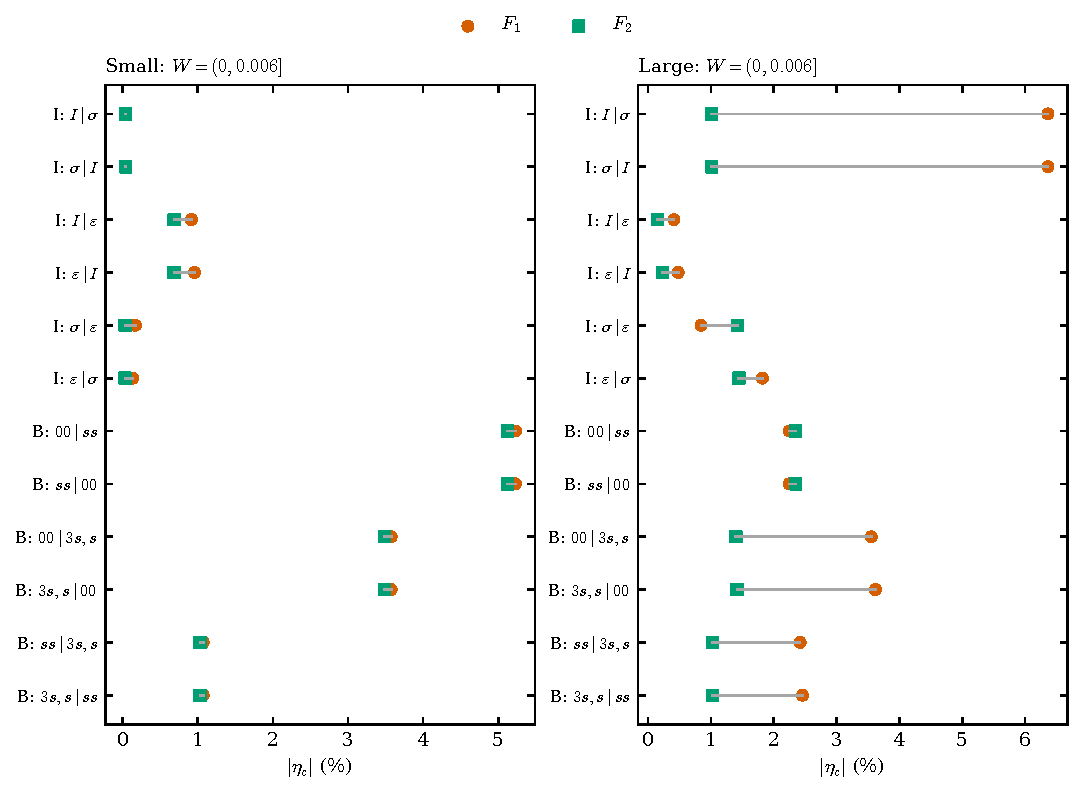
\includegraphics[width=.97\linewidth]{../figs/dense_shared_window.pdf}
\caption{A separate single-window diagnostic across all ordered pairs, using the current enlarged data and distinct from the adopted CFT-specific windows in Eq.~\eqref{eq:common-fit-windows}. I and B identify Ising and compact boson. A leftward shift from the circle ($F_1$) to the square ($F_2$) improves the leading coefficient. The same displayed interval and the same observations are used for both models; powers are fixed to the pair-specific manuscript values. Coefficients include powers of $\pi$, and $|\eta_c|$ is the absolute percentage discrepancy in Eq.~\eqref{eq:metrics}. The original largest sizes and $\ell=6,\ldots,10$ are retained.}
\label{fig:dense-shared}
\end{figure}
